%\documentclass[linenum,doublespace,onecolumn,draft]{SSA-SRL}



\documentclass[linenum]{SSA-SRL}

\citethisauthor{Zazueta ~M. and R.~Ortega}
% \vol{0}
% \iss{0}
\doi{00.0000/000000000}
\recdate{06 January 2025}

\newtheorem{proposition}{Proposition}
\usepackage{graphicx}
\begin{document}

\title{From Supersonic Events to Seismology: An Educational Framework Using Osiris-Rex for Calibration}

\author[1\orc{0000-0000-0000-0001}]{Marcela Zazueta}
\author[*1\orc{0000-0002-7741-0679}]{Roberto Ortega}


\affil[1]{CICESE-UALP, Centro de Investigacion Cientifica y de Educación Superior de Ensenada, Baja  California, Unidad Academica La Paz}{\auorc[https:// orcid.org/]{0000-0000-0000-0001}{(MZ)}\auorc{0000-0002-7741-0679}{(RO)}}
\corau{*Corresponding author: ortega@cicese.mx}


\begin{abstract}
This article aims to introduce undergraduate and postgraduate students to the study of seismic networks for detecting and analyzing supersonic events, such as meteorites or entrance capsules. By applying seismological techniques, specifically the analysis of arrival times, this study estimates the trajectory, angle, and theoretical impact of these events. While this approach has been documented in the literature for years, it has yet to become a widely adopted practice. In addition to traditional methodologies, we explore new potential approaches in a didactic manner\ref{}. The proliferation of seismic networks worldwide has resulted in an abundance of freely accessible data, offering significant opportunities to better understand observations of entrance of extraterrestrial sources. The methodology employed mirrors earthquake location techniques, the only difference is that instead of using the hypocenter, we use the epicenter as reference when we locate a bolide or capsule. To support learning and practical application, the study provides Jupyter notebook resources hosted in a publicly accessible repository. These tools are designed to serve as an educational gateway for those interested in applying seismological methods to the study of meteorites.

\end{abstract}
\maketitle
\section{Theoretical and Physical Insights}
\subsection{Introduction}
“I rarely look up, while you don’t even know how to look down. (Yo pa' arriba volteo muy poco, tu pa' abajo no sabes mirar)” It might sound like a conversation between seismologists and space scientists. In reality, it’s a lyric from a Mexican mariachi song that we should play at geophysics conferences.

Seismology, the study of seismic waves generated by earthquakes and other phenomena, has traditionally focused on understanding the Earth’s internal processes. However, its techniques and tools have broader applications, particularly in studying supersonic events such as meteorites entering the atmosphere. This paper explores the use of seismic networks to analyze and measure these high-velocity phenomena using global seismic data and established methodologies.

Meteorites and other supersonic objects produce characteristic seismic signals that can be analyzed using arrival times at multiple stations (e.g \citealp{Arrowsmith_2007,Berngardt_2015,de_Groot_Hedlin_2018,de_Groot_Hedlin_2014,Hedlin_2013,Pujol_2005,Qamar_1995,Stevanovi__2017,Brown_2003,
Edwards_2007,Edwards_2004}), similar to earthquake localization techniques \citep{Pujol_2006}. It is possible to estimate the trajectory and theoretical impact points of such objects using seismic data. Despite the conceptual exploration of this approach over the years, it remains underutilized in practice, offering an exciting avenue for educational and scientific exploration \citep{Silber_2024}.

The proliferation of seismic networks worldwide \citep{Ringler_2022} provides an unprecedented opportunity to engage students in this interdisciplinary field. These networks offer accessible, real-time data that can be used to connect theoretical concepts with practical applications. By introducing supersonic trajectory analysis as an extension of traditional seismology, we can inspire undergraduate and postgraduate students to explore novel uses of seismic networks, broadening their understanding of geophysics and its applications beyond the Earth’s surface \citep{KARAFYLLIDIS2024UNV}.

In this paper, we present a didactic framework for introducing students to the study of supersonic events using seismic data. The methodology parallels earthquake location techniques, focusing on arrival times, and velocity analysis. 

One of the key characteristics of studying this type of phenomenon is the dynamic nature of the source, which contrasts with earthquakes that have a single point of origin. In this case, the source is different at each time because the bolide is in motion. This movement, when projected at the surface, results in parabolic arrival time curves, rather than the circular patterns typical of an earthquake or an explosion, often referred to as a “burst” (\citealp {D_Auria_2006, Stevanovi__2017, Edwards_2004}).  We focus solely on the trajectory of the bolide in motion, as the reentry capsule did not explode or generated any burst-like event.

 We provide Jupyter notebooks \citep{7991618} hosted in a public repository, offering hands-on tools for data analysis and visualization. These resources are designed to guide students through the application of seismological techniques to meteorite tracking, fostering both scientific curiosity and practical skills.

It is important to say that seismic stations are not the only intruments that study moteorites and entry capsules, the vast majority are infrasound sensors (\citealp {Pilger_2018,Pilger_2020,Bond_r_2022,Gainville_2017,Jesus_2023,Kumar_2017,Stammler_2021}, even visual and cameras are good tools (\citealp{Arlt_2006,Borovi_KA_2003}).   By bridging seismology and supersonic phenomena, this study aims to demonstrate the versatility of seismic networks and inspire the next generation of researchers to think creatively about the applications of geophysical science.

In the following subsections, we will present two ways of solving a theoretical example of travel time calculation: vector projections \citep{Pujol_2005} and rotation matrices \citep{nagasawa_1978}. Both approaches reach the same equations. This exercise forms the foundation for a wide range of analytical possibilities, enabling students to solve a large number of exercises and apply the method in various ways. This exercise allows any motivated student of these topics to tackle problems that might otherwise seem abstract and unapproachable, offering a direct application of vector algebra and rotation tensors in a meaningful context. We will demonstrate this exercise as an introduction to our courses on the location of bolides and reentry capsules.

\subsection{\textbf{Background}}
One of the first articles on this topic was written by K. Nagasawa (\citeyear{nagasawa_1978}). Although the article is written in Japanese (Figure \ref{fig:nagasawa}), it serves as a true gateway to analyzing supersonic bolides through seismic networks. It is interesting to see analog seismograms with the equations that stand out in this work. Interestingly, despite the challenges to understand without any knowledge of Japanese, this article has opened the door to a comprehensive understanding of isochrones and the calculation of travel times. We even recommend replicating the formulas breaking the barriers of language. \cite{Ishihara_2004} presented an equation that describes the time from an origin to a seismic station, but it was based on \cite{nagasawa_1978} without proof. 


\vspace{0.5cm} 
\begin{figure} % 'H' para colocar la imagen exactamente donde se encuentra el código
    \centering
    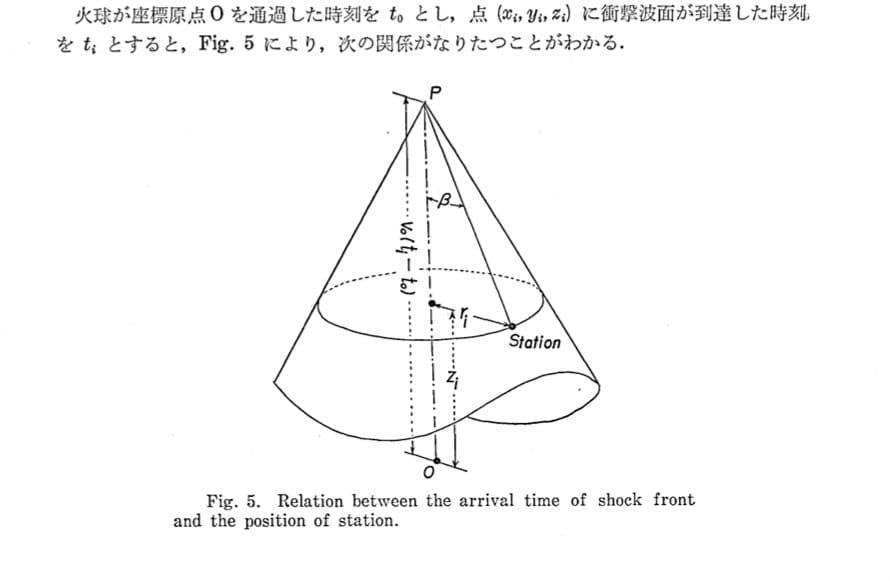
\includegraphics[width=0.6\textwidth]{Original79.jpeg} 
    \caption{Nagasawa's 1978 figure 5 that represented the travel time}
    \label{fig:nagasawa}
\end{figure}
\vspace{0.3cm} % Ajusta el espacio según sea necesario

Later, \cite{Pujol_2005} derived travel time equations using a straightforward approach based on the time from the origin of the shock wave to the station, dividing each component. \cite{Pujol_2005} rather than relying on rotations and distances for a geometric description, he preferred to show a simple path of the shock wave. We found both methods to be equally manageable (or challenging) for use in teaching materials.
There are also other expressions for the travel time that we will not explore, for example, those that follow a space shuttle that never lands \citep{Kanamori1992} or the travel time that resemble a nuclear explosion because only treats the bolide burst without analyzing trajectory. Also, there are some authors who use only graphical solutions without using travel-time equations (\citealp{Kalenda_2013, Brown_1996}). In addition, there are some networks that uses video cameras(\citealp{Ishihara_2004,Kereszturi_2021,Borovi_KA_2003}), It is worth noting that some authors have discussed the benefits of using graphical solutions as better methods for seismic location instead of travel time methods.\citep{https://doi.org/10.1029/2002GL014722}. 
\vspace{0.5cm} % Ajusta el espacio según sea necesario
%FIGURA 2
\begin{figure} % 'H' para colocar la imagen exactamente donde se encuentra el código
    \centering
    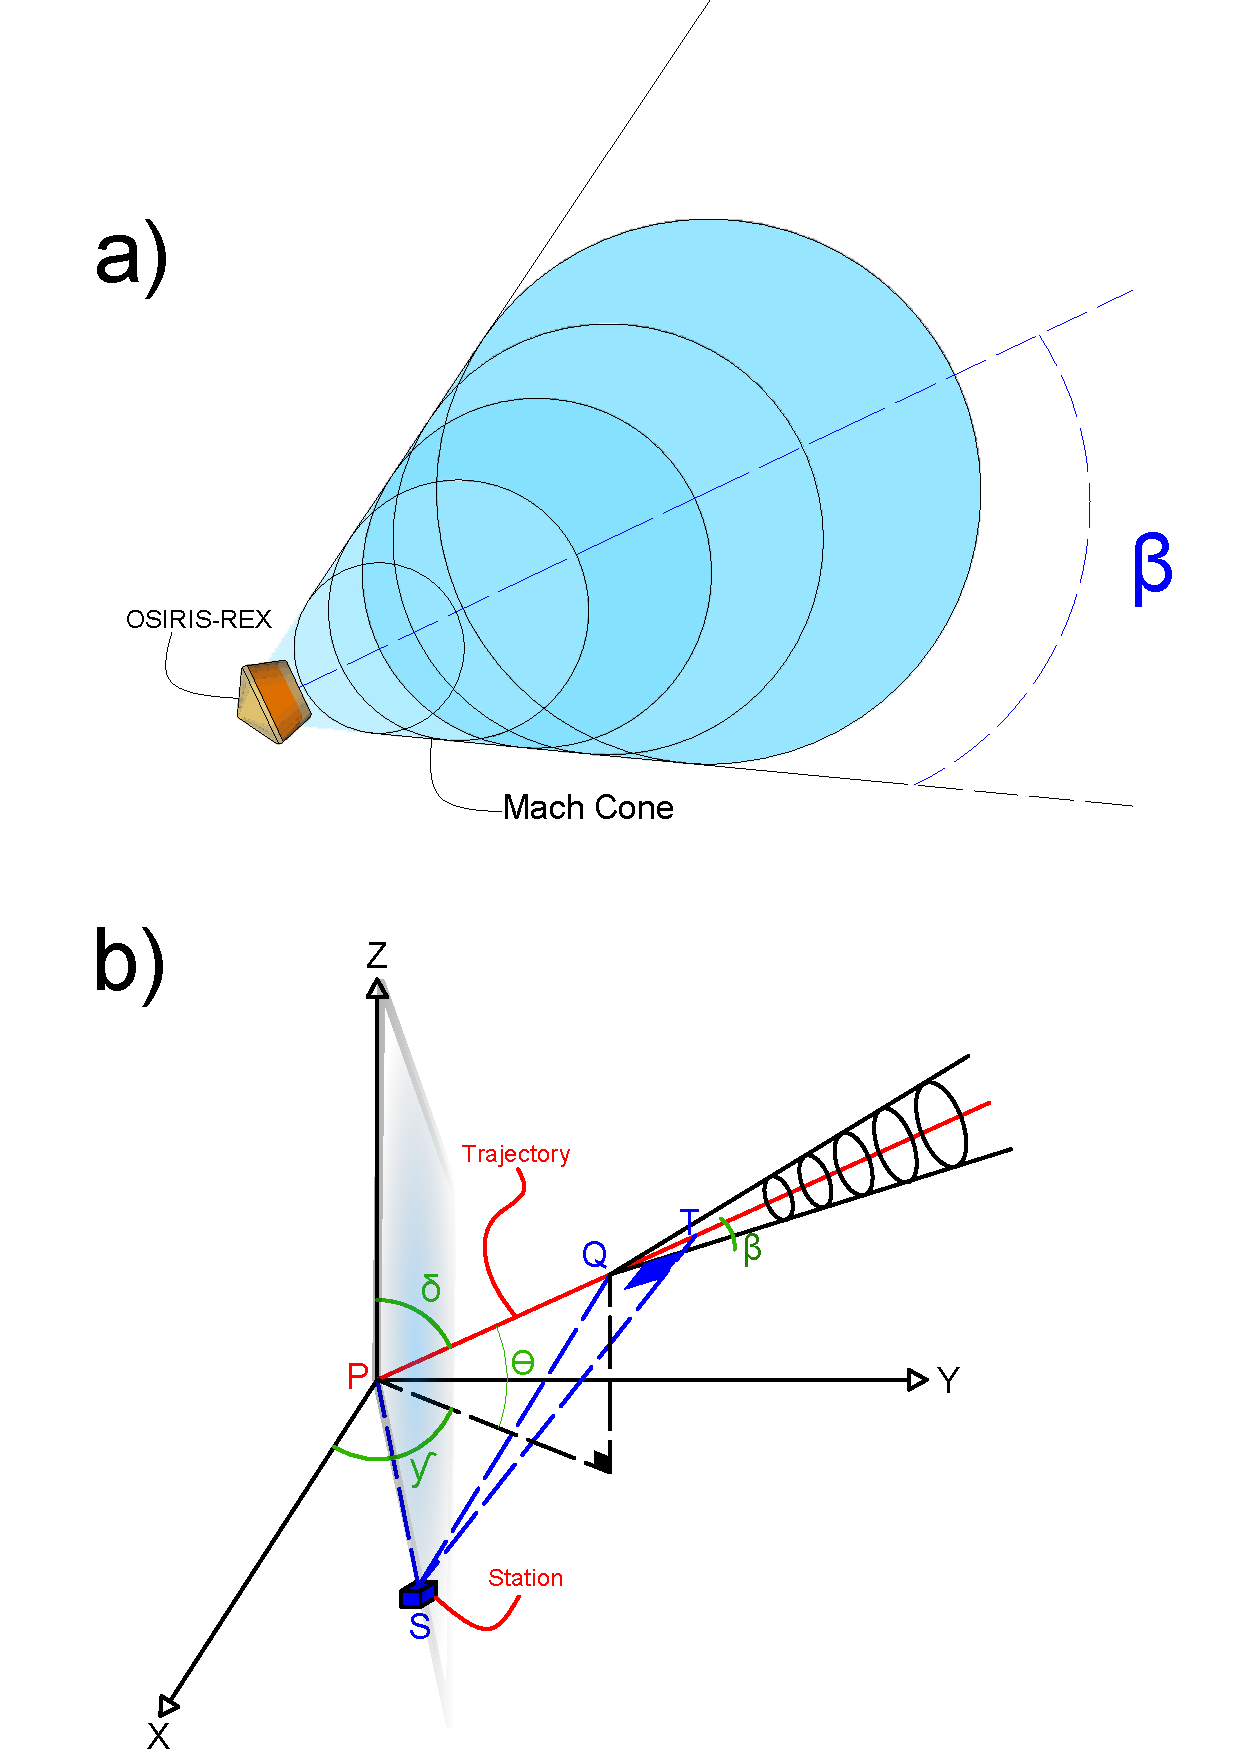
\includegraphics[width=0.4\textwidth]{PUJOL GENERAL2.pdf}
    \caption{a) schematizes the generation of the mach cone from the reentry of the SRC of the OSIRIS-REx mission and b) describes its geometry.}
    \label{fig:cono_osiris} % Etiqueta opcional para referenciar la imagen
\end{figure}
\vspace{0.2cm} % Ajusta el espacio según sea necesario

We took into account many considerations. For example, our approach is only valid for the projection where the Mach cone intersects the Earth’s surface, and we do not include the region where it extends beyond the trajectory. Additionally, we have not considered the explosive component, nor have we calculated changes in the projectile’s velocity, which will almost certainly occur when it enters the shallower regions of the atmosphere.

We have used constant values for both the projectile’s velocity and the speed of sound. This approximation is probably not valid for measurements that require detailed knowledge of such variations. Furthermore, we have not extended our work to geophysical studies, where seismic sensors could be used to better understand the effects occurring during ground interaction, such as coupling waves. Our focus has been solely on the first arrivals, which is similar to the approach in seismology where analysis is limited to the first arrivals of P-waves.

\subsection{\textbf{Methods}}
The Mach cone is fascinating and sparks interest in people in many ways. Since the goal is to determine the general characteristics of the trajectory of a bolide based on the arrival times of the shock wave associated with the Mach cone, as recorded by seismic stations, it is necessary to understand the basics of arrival times \citep{Pujol_2005}. Arrival times can be expressed as a summation of:
%EQ.1
\begin{equation}
t = t_0 - t_1 + t_2
\label{eq:time_calculation}
\end{equation}

where \( t_0 \) is the time when the bolide virtually impacts the surface, and \( t_1 \) is the time it takes for the bolide to travel from the point where the shock wave was generated to the impact point and \( t_2 \) is the last part. In fact, those previous considerations represent the wavefront that can be expressed at the speed of the bolide \( v \) and at the speed of sound \( c \), that actually represent \( t_0 \) and \( t_1 \) respectively. It is important to note that this representation differs from travel times in seismology where arrival times are measured from the origin time of the earthquake (hypocenter), not from the epicenter. In the case of a bolide's travel times, they are measured similarly to measuring times from the epicenter. 

In order to have travel times starting at the surface, \( t_1 \) needs to be adjusted and it is the reason why is negative in equation \ref{eq:time_calculation}, as it represents the time from the origin to the first impact. An interesting feature arises when the bolide directly impacts the seismic station (\( t_2 = 0 \)). If we use the impact time as the reference (\( t_0 = 0 \)), the total time \( t \) becomes negative (\( t = -t_1 \)). This is a special case where equation \ref{eq:time_calculation} has no solution. These details will become clearer in the following subsections as we develop the components that form equation \ref{eq:time_calculation}.
 
 Although there are multiple approaches to determine arrival times, they all lead to mathematically equivalent expressions. We will present these in a simple way in the following subsection. To visualize the geometry of the problem, we refer to the representations shown in Figure \ref{fig:cono_osiris} and Figure \ref{fig:geometría} \citep{Pujol_2005}.

In Figure \ref{fig:cono_osiris}, point \( P \) represents the impact location, which corresponds to the landing site of the object. Points \( Q \) and \( T \) are key points along the object's trajectory: \( Q \) is the vertex of the Mach cone only at the specific moment when the wave was generated, and \( T \) is the specific point where the wave was generated. We have used   Pujol's  2005 description. PQT and S remain fixed once the trajectory and location of the station are defined. This means, for instance, that Q will only be at the vertex of the cone at the moment the wave is generated, but moments later, Q will fall inside the cone as the system progresses.  The site \( S \) is the location of the station.

The angles \( \delta \) and \( \gamma \) represent the incidence angle and the azimuth of the trajectory, respectively. The angle \( \beta \) (Figure \ref{fig:cono_osiris}a) is a key feature of the Mach cone, defined as the angle between the object's trajectory and the wavefront of the cone (Figure \ref{fig:nagasawa}), from which we derive equation \ref{eq:mach_angle} \citep{maccoll__1937}.

%ECUACION 2
\begin{equation}
\sin \beta = \frac{c}{v} = \frac{1}{M}
\label{eq:mach_angle}
\end{equation}

Where \( v \) is the velocity of the object and \( c \) is the speed of sound. In our case, both \( v \) and \( c \) remain constant. The reasoning behind this method is based on calculating a series of distances that are then converted into times. 

\subsection{Vector projection and matrix rotation
}
\subsubsection{Vector projection}
We start with a known time, the impact at point \( P \),  and then, drawing backward along its trajectory to earlier points. In figure \ref{fig:geometría} we represented graphically the distances that are necessary to create the travel time using the vector projection approach. The important distances are the geographical location of the station $S$ and  $P$. There is also very important point: $Q$, where there are some graphical and physical characteristics. In essence Q  is the shortest distance from the line trajectory to the station. We also describe the point $W$ where the wave starts to travel only at the sound speed.  The travel time \(tt\) is:
\begin{equation}
tt =  \left( -\frac{PQ}{v}  + \frac{WS}{c} \right)
\label{eq:tt}
\end{equation}
and,
\begin{equation}
t= t_0 + tt.
\label{eq:t01}
\end{equation}

So, 
\begin{equation}
t = t_0 + \left( -\frac{PQ}{v}  + \frac{WS}{c} \right)
\label{eq:arrival time 1}
\end{equation}

Using the mathematical relations of figure \ref{fig:geometría}  and equation \ref{eq:mach_angle} we get:

\begin{equation}
t = t_0 + \frac{1}{v} \left(- PQ + \frac{QS}{\tan\beta} \right)
\label{eq:arrival time 1}
\end{equation}

We refer to \citep{Pujol_2005} for a detailed explanation on the derivation of equation \ref{eq:arrival time 1}. However, in a later subsection we used a simple relation that represents the relation of $-PQ + {QS}/{\tan\beta}$. This is the general expression for calculating the arrival time at station \( S \). 

It turns that the algorithm to solve equation \ref{eq:arrival time 1} is easy. Just using the following equations:
%GPO. DE ECUACIONES
%EQ.5
\begin{equation}
\mathbf{u} = (\cos \gamma \sin \delta, \sin \gamma \sin \delta, -\cos \delta)
\end{equation}
%EQ.6
\begin{equation}
\mathbf{b} = (x_s - x_0, \, y_s - y_0, \, z_s - z_0)
\end{equation}
\begin{flushleft}
\vspace{0.3cm} % Ajusta el espacio según sea necesario
%EQ.3
\begin{equation}
PQ = |\mathbf{b}| \cdot \cos(\alpha) = |\mathbf{b} \cdot \mathbf{u}|
\end{equation}
%EQ.4
\begin{equation}
QS = \sqrt{|\mathbf{b}|^2 - d_T^2}
\end{equation}


where $x_s$, $y_s$, $z_s$ = coordinates of the station, $x_0$, $y_0$, $z_0$ = coordinates of the virtual impact.

Analyzing equation \ref{eq:arrival time 1}, it is also a sum and subtraction of times, but expressed as ratios of distance to velocity.
%FIGURA 3
\begin{figure*}[t] 
    \centering
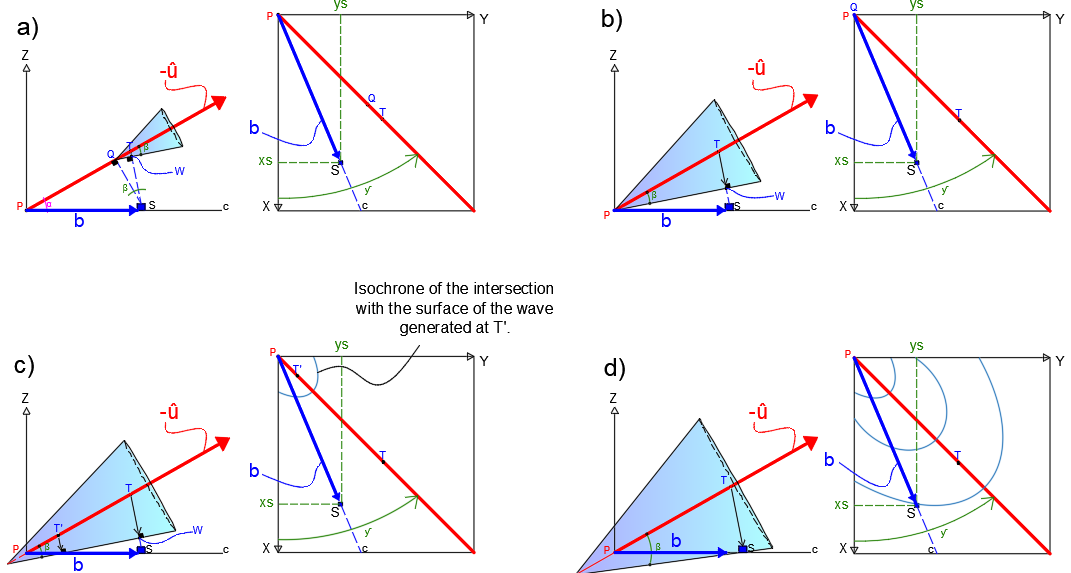
\includegraphics[width=1\textwidth]{DIAGRAMAS PUJOL 3.PNG} % Ajusta 'width' según el tamaño deseado
    \caption{Gemetric definition of arrival times and their surface projections at different times a) Generation of the bow wave b) Vertex of the cone impacting land, c) Generation of first isochrone and d) Shock wave reaching the station. At each moment, the cone is growing. The profile is projected in the Z-P-S plane of Figure \ref{fig:cono_osiris} }
    \label{fig:geometría} % Etiqueta opcional para referenciar la imagen
\end{figure*}
\vspace{0.5cm} % Ajusta el espacio según sea necesario


\begin{figure*}[t] % 'H' para colocar la imagen exactamente donde se encuentra el código
    \centering
    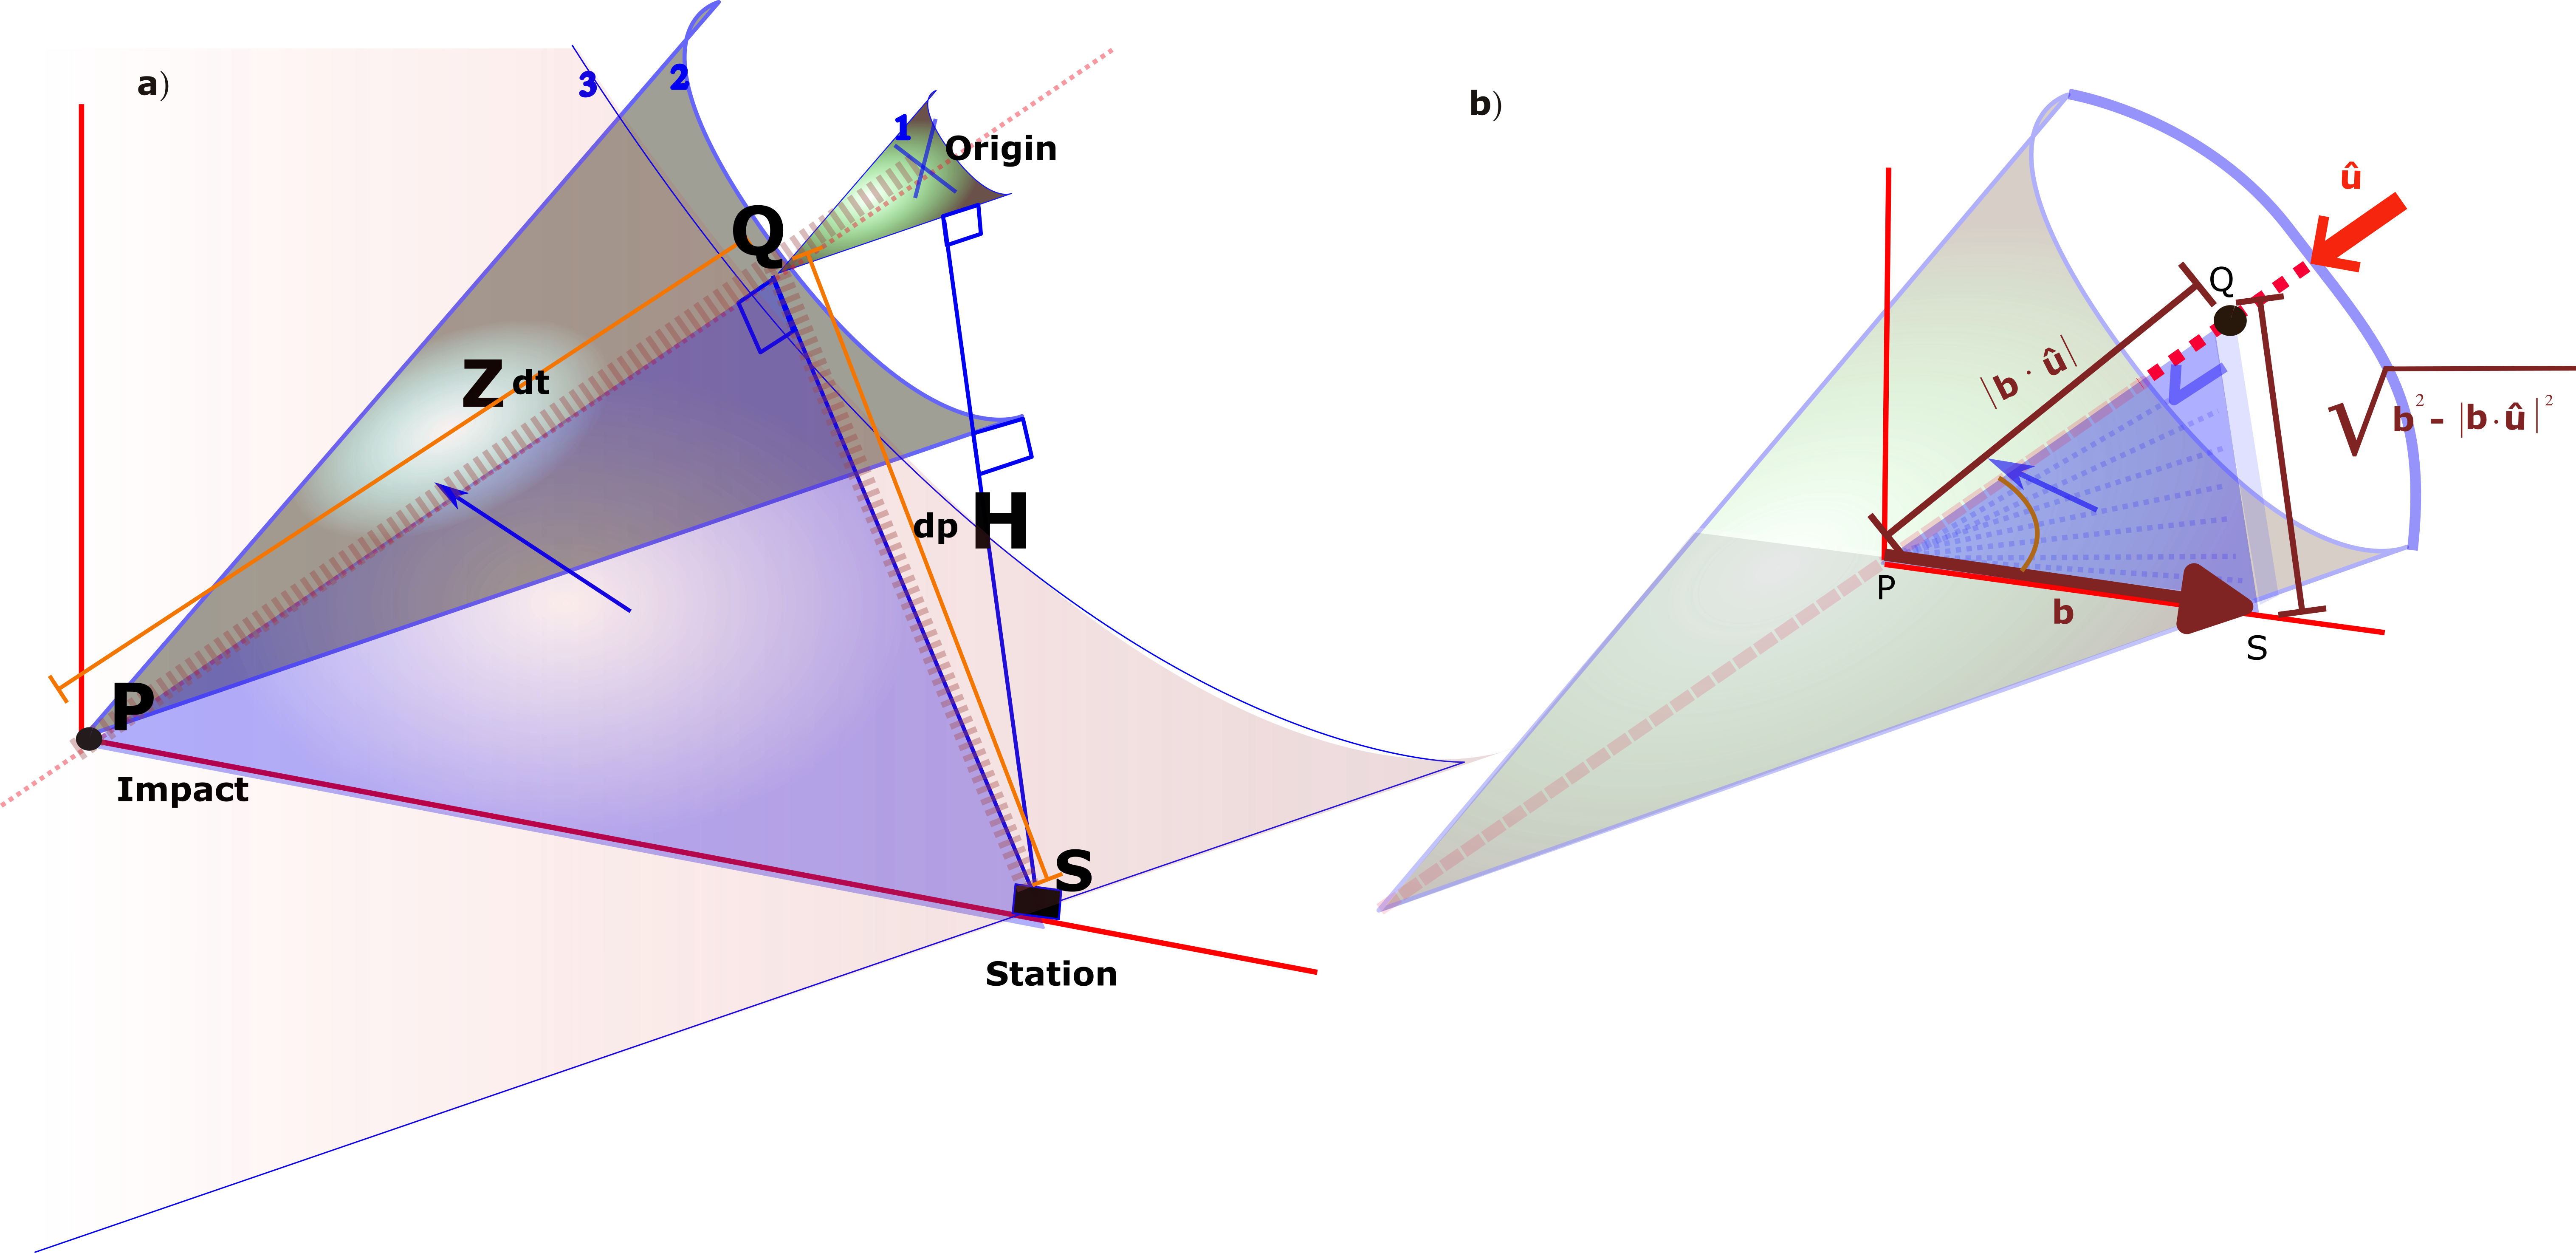
\includegraphics[width=1\textwidth]{version3Dnueva.png} % Ajusta 'width' según el tamaño deseado
    \caption{3D representation of the two stages of arrival time construction: 
(a) First stage, considering the beta angle ($\beta$) in the construction of the Mach cone, independent of the inclination and trajectory. 
(b) Second stage, description of distances based on the trajectory projections, using the horizontal as a reference. 
Both stages can also be represented using a rotation tensor.}
    \label{fig:3dpujol} % Etiqueta opcional para referenciar la imagen
\end{figure*}
Also, figure \ref{fig:geometría} shows the isochrones, which result from the intersubsections of the Mach cone with the surface (Figures \ref{fig:geometría}c and \ref{fig:geometría}d). 

However, vector projection is not the only or definitive form; there is a much more general approach tha we will also consided through a series of geometric considerations, leads to the following expression \cite{Ishihara_2004}:

\begin{equation}
t = t_0 + \frac{1}{v} \left( -Z' + \frac{\sqrt{X'^2 + Y'^2}}{\tan\beta} \right)
\end{equation}
So, we will connect both approaches  


\subsubsection{Graphical representation of the vector projection and matrix rotation}

The process mach cone construction of the shock wave propagation is represented in figure \ref{fig:3dpujol}

\begin{itemize}
    \item \textbf{Initiation of the Shock Wave:} First,  In Figure \ref{fig:3dpujol}a (Cone 1), the \textit{shock wave} is generated at the origin. This wave propagates toward station \( S \), and simultaneously, the Mach cone begins to form. The \textit{normal} to the Mach cone indicates the shortest path between the cone and the station.

    \item \textbf{Vertex Impact on the Surface:} When the vertex of the Mach cone reaches the surface (Figure \ref{fig:3dpujol}a ,Cone 2), , the \textit{shock wave} stops propagating underground. However, for explanatory purposes, the cone is still illustrated as advancing through the atmosphere, where it continues to expand.

    \item \textbf{Arrival of the Shock Wave at the Station:} Finally, the \textit{shock wave} reaches station \( S \) (Figure \ref{fig:3dpujol}a ,Cone 3). 

This process can be divided into two key travel distances:
    \begin{itemize}
        \item \textit{Initial travel distance (QP):} The path from the origin to the impact point \( P\).
        \item \textit{Distance from the vertex Q to the station S: QS} The final segment of the propagation path.
    \end{itemize}
\end{itemize}

These two distances are critical for calculating the total travel path of the \textit{shock wave} through the system. The  (\( PS \)) is the geographic distance that serves as the basis for these calculations. Second, the representation of distances using vector projection and matrix rotation can be summarized as:
\begin{itemize}
    \item \( P-Q: \) Distance between the origin point \( Q \) and the impact point \( P \).
    \item \( Q-S: \) Distance between the \( Q \)  point and station \( S \).2
\end{itemize}

Both distances can be calculated using two main methods:

\begin{enumerate}
    \item \textbf{Vector Projection Method:} This method directly constructs the projections of the vertices of the triangle \( P-Q-S \) onto a coordinate system. As explained in the previuos subsection. It is a straightforward, geometric approach based on simple projections.  

    \item \textbf{Matrix Rotation Method:} This approach uses a rotation matrix to transform the \( P-Q-S \) from an initial frame of reference  (cone vertical) to its final inclination. The rotation matrix acts on the coordinate data \( (X, Y, Z) \). The purpose of this method is to rotate the Mach cone and represent the data at its final inclination. This rotation provides a generalized way to project data in three-dimensional space.
   
\end{enumerate}

 While the \textbf{vector projection method} builds the distances directly from the triangle vertices, the \textbf{matrix rotation method} transforms the data through geometric rotations, allowing for a more general representation of the \textit{shock wave} path.


\subsubsection{Rotations}
The method consists of transforming the trajectory (represented by \( P-Q-S \) in the previous method) into a more convenient coordinate system by rotating the global reference system \( X', Y', Z' \) \cite{Ishihara_2004}. This is done using the incidence and azimuth angles of the trajectory, with a slight difference in how the azimuth angle is considered—using its complementary angle, \( \theta \) (Figure \ref{fig:geometría}). From this, we derive the individual rotation matrices around the \( Z \)-axis (azimuth) and \( Y \)-axis (incidence):

\vspace{0.4cm}
\begin{equation}
R_z = 
\begin{bmatrix}
-\cos{\gamma} & -\sin{\gamma} & 0 \\
\sin{\gamma} & \cos{\gamma} & 0 \\
0 & 0 & 1
\end{bmatrix}
\end{equation}

\vspace{0.4cm} % Ajusta el espacio según sea necesario

\begin{equation}
R_y = 
\begin{bmatrix}
-\sin{\theta} & 0 & -\cos{\theta} \\
0 & 1 & 0 \\
-\cos{\theta} & 0 & \sin{\theta}
\end{bmatrix}
\end{equation}

\vspace{0.4cm} % Ajusta el espacio según sea necesario

It follows that we get the rotation matrix:

\vspace{0.5cm}

\begin{equation}
M_R = 
\begin{bmatrix}
\cos(\gamma) \cdot \sin(\theta) & \sin(\gamma) \cdot \sin(\theta) & -\cos(\theta) \\
-\sin(\gamma) & \cos(\gamma) & 0 \\
\cos(\gamma) \cdot \cos(\theta) & \sin(\gamma) \cdot \cos(\theta) & \sin(\theta)
\end{bmatrix}
\end{equation}
 % Ajusta el espacio según sea necesario


%Finalmente la trayectoria está dada por:\\
\vspace{0.4cm}
Finally the trajectory is: 

\begin{equation}
\begin{bmatrix}
X' \\ 
Y' \\ 
Z'
\end{bmatrix}
=
M_R \cdot \mathbf{b}_m
\end{equation}

\vspace{0.4cm} % Ajusta el espacio según sea necesario

where:

\vspace{0.4cm} % Ajusta el espacio según sea necesario

\begin{equation}
\mathbf{b}_m =
\begin{bmatrix}
x_s - x_0 \\
y_s - y_0 \\
z
\end{bmatrix}
\end{equation}

\vspace{0.4cm} % Ajusta el espacio según sea necesario

\begin{equation}
\theta = 90^\circ - \gamma
\end{equation}

This method is more general because it allows working with any reference system. 

%FIGURA 4
\begin{figure*}[t] % 'H' para colocar la imagen exactamente donde se encuentra el código
    \centering
    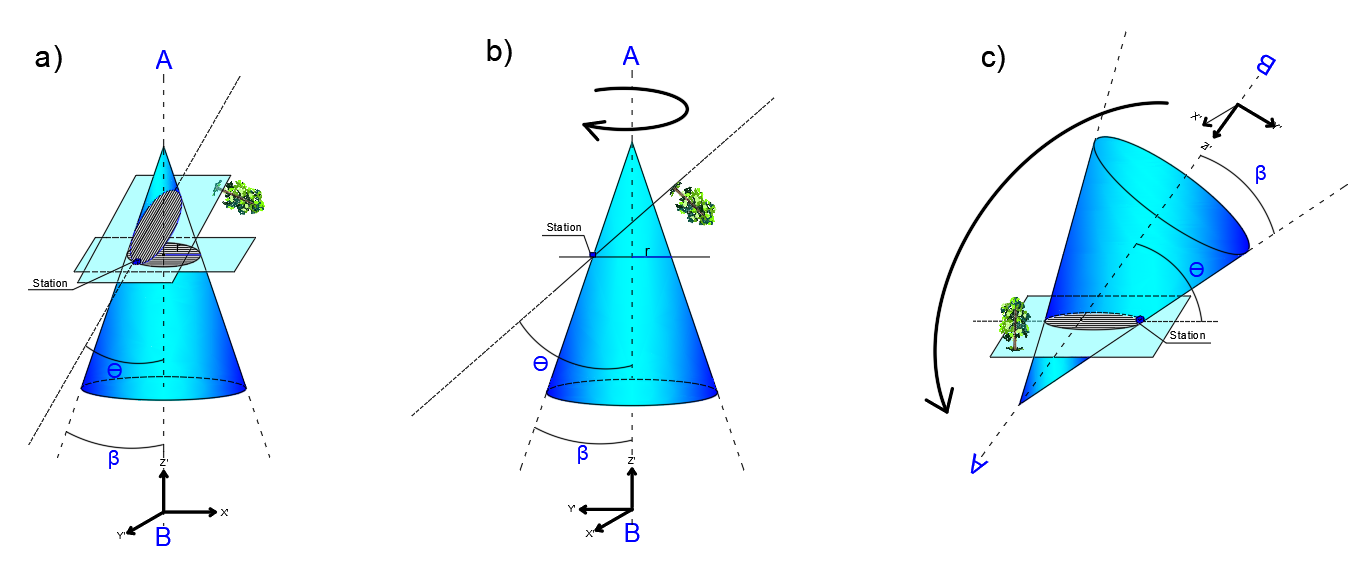
\includegraphics[width=0.8\textwidth]{CONOS.PNG} % Ajusta 'width' según el tamaño deseado
    \caption{Three-dimensional representation of the cone and its intersubsection with different planes. In (a), the inclined cone intersects the earth's surface; in (b), it is positioned vertically to appreciate the inclination of the cutting plane with respect to the cone; and in (c), an additional horizontal plane perpendicular to the axis of the cone is introduced as a comparison between both planes.}
    \label{fig:mi_imagen} % Etiqueta opcional para referenciar la imagen
\end{figure*}
\end{flushleft}

\subsection{Examples, discussion and results}


The reentry of the SRC (Sample Return Capsule) from the OSIRIS-REx mission represented an event of great interest to the scientific community, offering a unique opportunity to study a phenomenon analogous to the entry of a meteorite into the atmosphere. This reentry was one of the most extensively instrumented, thanks to a collaborative campaign involving researchers from various institutions who strategically deployed geophysical instruments to analyze the event. 

However, we are aware that seismic data will be released to the general scientific community in the near future, so only very limited data is available at the time of writing this article, limiting the practical application of the proposed methods. Despite this, the purpose of this work remains educational, aiming to incorporate the records into future analyses once they become available.

At first glance, it may seem like a trivial exercise, resolved simply through angles and distances. However, after working with the equations, we find that the phenomenon is difficult to understand because the source is moving at a speed greater than the speed of sound, making it a challenge for individuals with seismological training (RO). 

In contrast, it is very encouraging that students can have their first encounter with seismology through the study of supersonic bolides by analyzing \( N \)-wave arrivals at seismic stations (MZ).

%\citep{Hedlin_2010}
%citep{Langston_2004}
%\citep{Ishihara_2004}
%\citep{Olivieri_2023}
%\citep{Silber_2024}
%\citep{D_Auria_2006}
%\citep{Stevanovi__2017}
%\citep{Qamar_1995}
%\citep{Tapia_2016}
%\citep{Blom_2024}
%\citep{Hedlin_2013}
%\citep{Henneton_2015}
%\citep{EDWARDS_2004}
%\citep{Berngardt_2015}
%citep{Ishihara_2014}
%\citep{de_Groot_Hedlin_2008}
%\citep{Kalenda_2013}
%\citep{Ishihara_2014}
%\citep{Ishihara_2012}
%\citep{Edwards_2008}
%\citep{Pujol_2005}
%\citep{Arrowsmith_2007}
%\citep{Manville_2004}
%\citep{REVELLE_1997}
%\citep{Brown_2002}
%\citep{Edwards_2007}
%\citep{PICHON_2008}
%\citep{Kereszturi_2021}
%\citep{Seleznev_2014}
%\citep{BROWN_2003}
%\citep{REVELLE_2004}
%\citep{Silber_2023}
%\citep{Kumar_2017}
%\citep{de_Groot_Hedlin_2018}
%\citep{Wilson_2019}
%\citep{Daubar_2018}
%\citep{de_Groot_Hedlin_2018}
%\citep{McFadden_2021}
%\citep{Yamada_2012}
%\citep{D_Auria_2006}
%\citep{Borovi_ka_2015}
%\citep{Edwards_2006}
%\citep{Stammler_2021}
%\citep{Bond_r_2022}
%\citep{Ben_Menahem_1975}
%\citep{Yamada_2012}
%\citep{Campus_2009}
%\citep{Silber_2018}
%\citep{SPURN__2010}
%\citep{Karakostas_2024}
%\citep{Koper_2002}
%\citep{Green_2009}
%\citep{Pilger_2020}
%\citep{BLOM_2024}
%\citep{de_Groot_Hedlin_2009}
%\citep{Silber_2023}
%\citep{Millet_2010}
%\citep{Arlt_2006}
%\citep{Edwards_2009}
%\citep{Nippress_2017}
%\citep{ReVelle_2007}
%\citep{Gritsevich_2008}
%\citep{Gainville_2017}
%\citep{BROWN_1996}
%\citep{Karakostas_2018}
%\citep{Evers_2018}
%\citep{Ruzhin_2014}
%\citep{Hicks_2023}
%\citep{Pujol_2006}
%\citep{de_Groot_Hedlin_2014}
%\citep{P_sztor_2023}
%\citep{Asming_2022}
%\citep{Tancredi_2009}
%\citep{Blanc_2009}
%\citep{Yasyukevich_2024}
%\citep{ReVelle_2009}
%\citep{BOROVI_KA_2003}
%\citep{McKenna_2005}
%\citep{ReVelle_2006}
%\citep{ReVelle_2007}
%\citep{Meschede_2011}
%\citep{Froment_2020}
%\citep{Poklad_2018}
%\citep{Bishop_2022}
%\citep{Cordero_2011}
%\citep{Norris_2009}
%\citep{Lognonn__2016}
%\citep{Albert_2023}
%\citep{Jesus_2023}
%\citep{ReVelle_2007}
%\citep{Ackerley_2022}
%\citep{Krasnov_2006}
%\citep{Ruzhin_2014}
%\citep{Nan_Zou_2009}
%\citep{Stump_2012}
%\citep{Pilger_2018}
%\citep{1996}
%\citep{Blom_2018}
%\citep{Mead_2023}
%\citep{Sekanina_1983}
%\citep{Spurn__2020}
%\citep{Kulichkov_2018}
%\citep{ReVelle_1996}
%\citep{Sabatini_2016}
%\citep{2022}
%\citep{Albert_2019}
%\citep{Sabatini_2018}
%\citep{Sheikh}
%\citep{Brown_2008}
%\citep{Donn_1964}
%\citep{Gounelle_2006}
%\citep{Hardin_2002}
%\citep{de_Larquier_2010}
%\citep{Hayne_2018}

%\begin{itemize}
%\item \verb"\citethisauthor{First, A.,"
%            \verb"A. Second, and A. Third}"
%\item \verb"\vol{2}"
%\item \verb"\iss{1}"
%\item \verb"\doi{00.0000/0000000000}"
%\item \verb"\recdate{00 Month 0000}"
%\end{itemize}



%\begin{proposition}
%Here is the body of the preposition...
%\end{proposition}


\begin{datres}%[CUSTOM HEAD]
Here is the content of Data and Resources.
\end{datres}

\subsection{Declaration of Competing Interests}

The authors acknowledge that there are no conflicts of interest recorded.\footnote{The authors acknowledge that there are no conflicts of interest recorded.}

\begin{ack}%[CUSTOM ACK HEAD]
%We thank Dr. Jose Pujol, who has given us access to his original códigos. Agradecemos a CICESE UALP y CONHACYT por el apoyo. 

We thank Dr. Jose Pujol for providing access to his original codes. We also thank CICESE, UALP, and CONACYT for their support.
\end{ack}

\bibliography{citations.bib}

\end{document}


\citep{Hedlin_2010}
\citep{Langston_2004}
\citep{Ishihara_2004}
\citep{Olivieri_2023}
\citep{Silber_2024}
\citep{D_Auria_2006}
\citep{Stevanovi__2017}
\citep{Qamar_1995}
\citep{Tapia_2016}
\citep{Blom_2024}
\citep{Hedlin_2013}
\citep{Henneton_2015}
\citep{EDWARDS_2004}
\citep{Berngardt_2015}
\citep{Ishihara_2014}
\citep{de_Groot_Hedlin_2008}
\citep{Kalenda_2013}
\citep{Ishihara_2014}
\citep{Ishihara_2012}
\citep{Edwards_2008}
\citep{Pujol_2005}
\citep{Arrowsmith_2007}
\citep{Manville_2004}
\citep{REVELLE_1997}
\citep{Brown_2002}
\citep{Edwards_2007}
\citep{PICHON_2008}
\citep{Kereszturi_2021}
\citep{Seleznev_2014}
\citep{BROWN_2003}
\citep{REVELLE_2004}
\citep{Silber_2023}
\citep{Kumar_2017}
\citep{de_Groot_Hedlin_2018}
\citep{Wilson_2019}
\citep{Daubar_2018}
\citep{de_Groot_Hedlin_2018}
\citep{McFadden_2021}
\citep{Yamada_2012}
\citep{D_Auria_2006}
\citep{Borovi_ka_2015}
\citep{Edwards_2006}
\citep{Stammler_2021}
\citep{Bond_r_2022}
\citep{Ben_Menahem_1975}
\citep{Yamada_2012}
\citep{Campus_2009}
\citep{Silber_2018}
\citep{SPURN__2010}
\citep{Karakostas_2024}
\citep{Koper_2002}
\citep{Green_2009}
\citep{Pilger_2020}
\citep{BLOM_2024}
\citep{de_Groot_Hedlin_2009}
\citep{Silber_2023}
\citep{Millet_2010}
\citep{Arlt_2006}
\citep{Edwards_2009}
\citep{Nippress_2017}
\citep{ReVelle_2007}
\citep{Gritsevich_2008}
\citep{Gainville_2017}
\citep{BROWN_1996}
\citep{Karakostas_2018}
\citep{Evers_2018}
\citep{Ruzhin_2014}
\citep{Hicks_2023}
\citep{Pujol_2006}
\citep{de_Groot_Hedlin_2014}
\citep{P_sztor_2023}
\citep{Asming_2022}
\citep{Tancredi_2009}
\citep{Blanc_2009}
\citep{Yasyukevich_2024}
\citep{ReVelle_2009}
\citep{BOROVI_KA_2003}
\citep{McKenna_2005}
\citep{ReVelle_2006}
\citep{ReVelle_2007}
\citep{Meschede_2011}
\citep{Froment_2020}
\citep{Poklad_2018}
\citep{Bishop_2022}
\citep{Cordero_2011}
\citep{Norris_2009}
\citep{Lognonn__2016}
\citep{Albert_2023}
\citep{Jesus_2023}
\citep{ReVelle_2007}
\citep{Ackerley_2022}
\citep{Krasnov_2006}
\citep{Ruzhin_2014}
\citep{Nan_Zou_2009}
\citep{Stump_2012}
\citep{Pilger_2018}
\citep{1996}
\citep{Blom_2018}
\citep{Mead_2023}
\citep{Sekanina_1983}
\citep{Spurn__2020}
\citep{Kulichkov_2018}
\citep{ReVelle_1996}
\citep{Sabatini_2016}
\citep{2022}
\citep{Albert_2019}
\citep{Sabatini_2018}
\citep{Sheikh}
\citep{Brown_2008}
\citep{Donn_1964}
\citep{Gounelle_2006}
\citep{Hardin_2002}
\citep{de_Larquier_2010}
\citep{Hayne_2018}














